% Uncomment this to make slides with overlays:
%\documentclass[slides]{beamer}

% Uncomment these (but comment the above \documentclass line) to make handouts:
\documentclass[handout]{beamer}

% Uncomment these to have more than one slide per page
\usepackage{pgfpages}
\pgfpagesuselayout{2 on 1}[border shrink=5mm]
\pgfpageslogicalpageoptions{1}{border code=\pgfusepath{stroke}}
\pgfpageslogicalpageoptions{2}{border code=\pgfusepath{stroke}}

\usepackage[]{graphicx, color, hyperref}

\mode<presentation>
{
	%\usetheme[secheader]{Boadilla}
	%\usecolortheme[rgb={.835, .102,.169}]{structure}  
	\usetheme[width= 0cm]{Goettingen}
	%\setbeamercovered{transparent}
}
\setbeamertemplate{navigation symbols}{}
\setbeamertemplate{footline}[frame number]

\definecolor{blue2}{rgb}{0.278,0.278,0.729} 
\newcommand{\blue}[1]{\textcolor{blue2}{#1}}
\newcommand{\white}[1]{\textcolor{white}{#1}}
\newcommand{\red}[1]{\textcolor{red}{#1}}
\newcommand{\xbar}{\overline{x}}
\newcommand{\ybar}{\overline{y}}
\newcommand{\phat}{\widehat{p}}
\newcommand{\prob}{\mbox{Pr}}
\newcommand{\E}{\mathbb{E}}
\newcommand{\Var}{\mbox{Var}}
\newcommand{\cp}{\oplus}
\newcommand{\cm}{\circleddash}


\title{Lecture 24: Linear Regression Part I}
\author{Chapter 7.1-7.2}
\date{}


\begin{document}
%------------------------------------------------------------------------------
\begin{frame}
\titlepage
\end{frame}
%------------------------------------------------------------------------------


%------------------------------------------------------------------------------
\begin{frame}[fragile]
\frametitle{Questions for Today}

Say we have the height/weight of 50 individuals and we display the scatterplot/bivariate plot of the seemingly \blue{linear} relationship:
\begin{center}
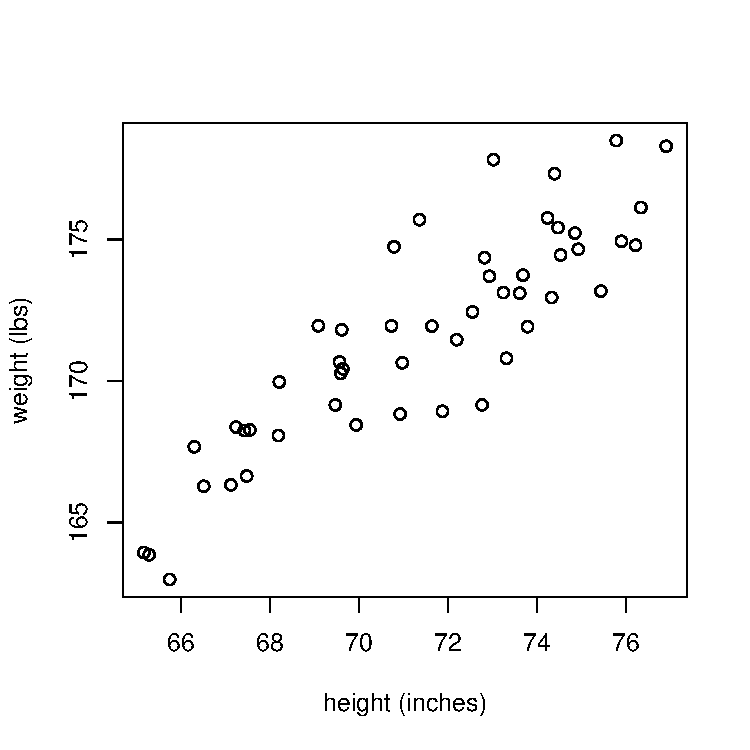
\includegraphics[height=5cm]{figure/lec24-002.pdf}
\end{center}
\pause Questions:  
\begin{itemize}
\item What is the ``best'' fitting line through these points?
\item What do we mean by ``best''?
\end{itemize}

\end{frame}
%------------------------------------------------------------------------------


%------------------------------------------------------------------------------
\begin{frame}[fragile]
\frametitle{Regression}
There are many types of \blue{regression}, all in order to estimate the relationship between variables.  
%
% Comment this
%
\vspace{0.5cm}
\pause We start by considering \blue{simple linear regression (SLR)}:
\begin{itemize}
\item a single \blue{explanatory variable / independent variable / predictor variable} $x$
\item an \blue{outcome variable / dependent variable} $y$
\item a presumed linear relationship between them
\end{itemize}

\end{frame}
%------------------------------------------------------------------------------


%pdf("./11.2 Linear Regression/nonlinear.pdf", width=5, height=5)
%x <- seq(0, 2, by=0.05)
%f <- function(x){
%  x*(2-x)
%}
%plot(x, f(x), xlab="# of corn plants per sq mile (1000s)",
%     ylab="corn yield per sq mile (in bushels)")
%dev.off()
%------------------------------------------------------------------------------
\begin{frame}[fragile]
\frametitle{Example of Non-Linear Relationship}
At first as you plant more corn plants, you have higher yield, but past a certain point plants fight for limited resources and they die. 
\begin{center}
\pause 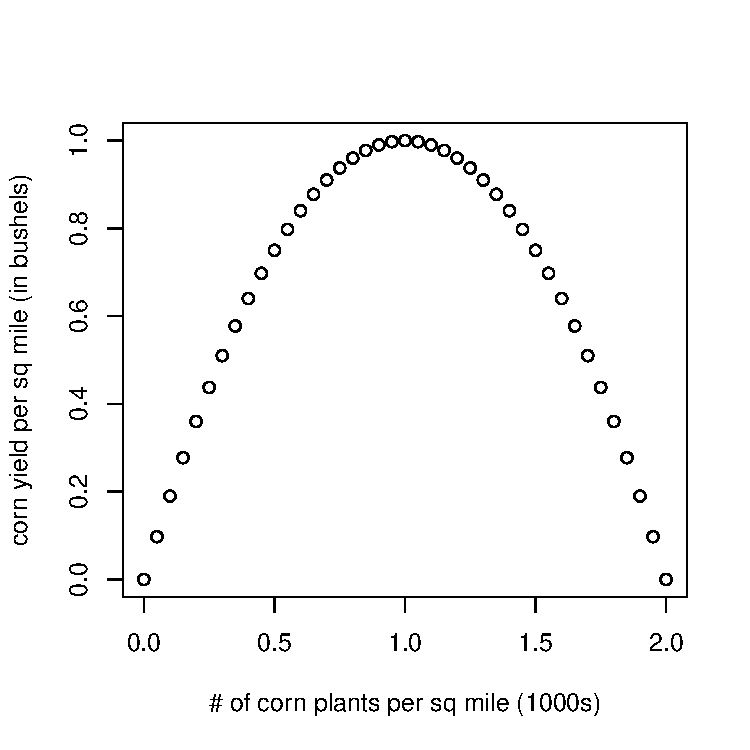
\includegraphics[width=0.6\textwidth]{figure/nonlinear.pdf}
\end{center}
   
\end{frame}
%------------------------------------------------------------------------------


%-------------------------------------------------------------------------------
\begin{frame}
\frametitle{Modeling $x$ and $y$ Linearly}
%
% Comment this
%
The \blue{SLR model} assumes that the relationship between $x$ and $y$ can be modeled by a line:
\begin{eqnarray*}
y &=& \beta_0 + \beta_1 x
\end{eqnarray*}
where 
\pause\begin{itemize}
\item $\beta_0$ is the unknown \blue{intercept parameter}
\item $\beta_1$ is the unknown \blue{slope parameter}
\end{itemize}

\end{frame}
%-------------------------------------------------------------------------------


%-------------------------------------------------------------------------------
\begin{frame}
\frametitle{Procedure}
%
% Comment this
%
Based on $n$ pairs of observations $(x_i, y_i)$
\begin{enumerate}
\pause\item Compute \blue{point estimates}
\begin{itemize}
\item $b_0$ of parameter $\beta_0$
\item $b_1$ of parameter $\beta_1$
\end{itemize}
\pause\item Associate standard errors $SE_{b_0}$ and $SE_{b_1}$
\pause \item For both the intercept and slope
\begin{itemize}
\item Build confidence intervals
\item Do hypothesis test
\begin{eqnarray*}
&& H_0: \beta = 0\\
\mbox{vs}&& H_A: \beta \neq 0 
\end{eqnarray*}
\end{itemize}
\end{enumerate} 
\pause 
The equation
\[
\widehat{y} = b_0 + b_1 x
\]
is called the \blue{least squares line} where $\widehat{y}$ is the \blue{fitted/predicted value}. %You can also think of it as an \blue{average} y-value for the given $x$.
\end{frame}
%-------------------------------------------------------------------------------


%-------------------------------------------------------------------------------
\begin{frame}
\frametitle{Fitted Value}
Here $\widehat{y} = 100 + 0.99 x$.  Thus for $x=73$, $\widehat{y}=173.22$:
\begin{center}
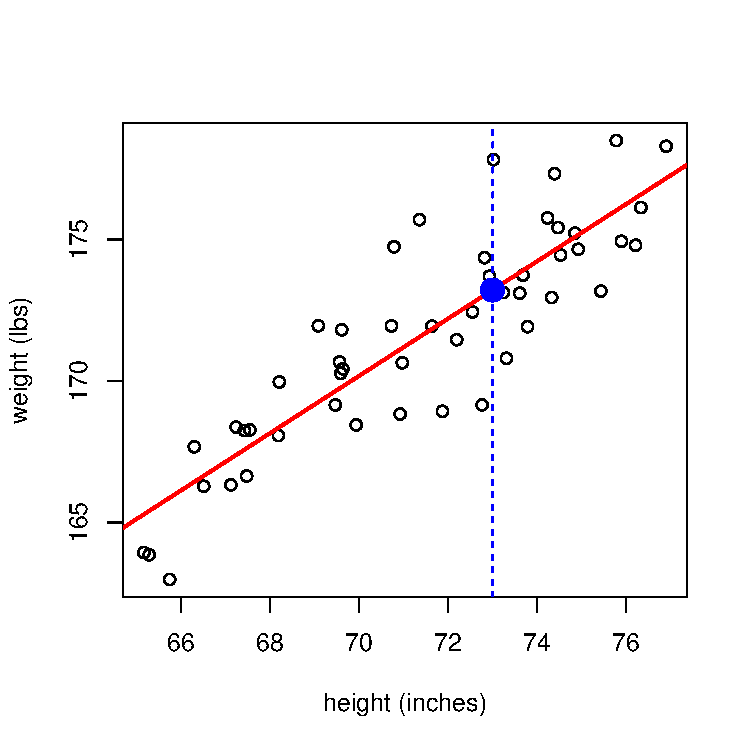
\includegraphics[width=0.7\textwidth]{figure/average.pdf}
\end{center}
\end{frame}
%-------------------------------------------------------------------------------


%-------------------------------------------------------------------------------
\begin{frame}
\frametitle{Residuals}
%
% Comment this
%
\blue{Residuals} are what's leftover:  leftover variation in the data unexplained by the model:  
\pause
\begin{eqnarray*}
\mbox{Residual} &=& \mbox{Data} - \mbox{Fit} \\
e_i &=& y_i - \widehat{y}_i
\end{eqnarray*}
where $e_i$ is the \blue{residual} of the $i^{th}$ observation $(x_i, y_i)$.

\vspace{0.5cm}
\pause We can think of the $e_i$'s as \blue{deviations} from the model.  The smaller the deviations, the better the fit.  
\end{frame}
%-------------------------------------------------------------------------------


%-------------------------------------------------------------------------------
\begin{frame}
\frametitle{Residual Plot}
Residual plots: take previous plot and flatten the red line by subtracting $\widehat{y}$ from $y$.

\begin{center}
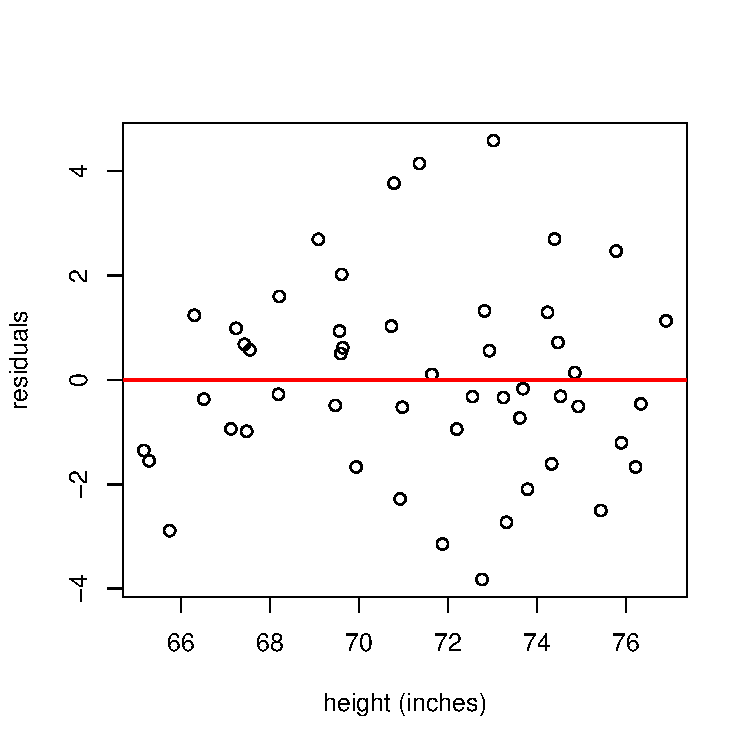
\includegraphics[width=0.7\textwidth]{figure/residuals.pdf}
\end{center}

\end{frame}
%-------------------------------------------------------------------------------


%-------------------------------------------------------------------------------
\begin{frame}
\frametitle{Correlation Coefficient}

The correlation coefficient $R$ is a value between $[-1, 1]$ that measures the strength of the linear relationship between $x$ and $y$.  

\begin{center}
\pause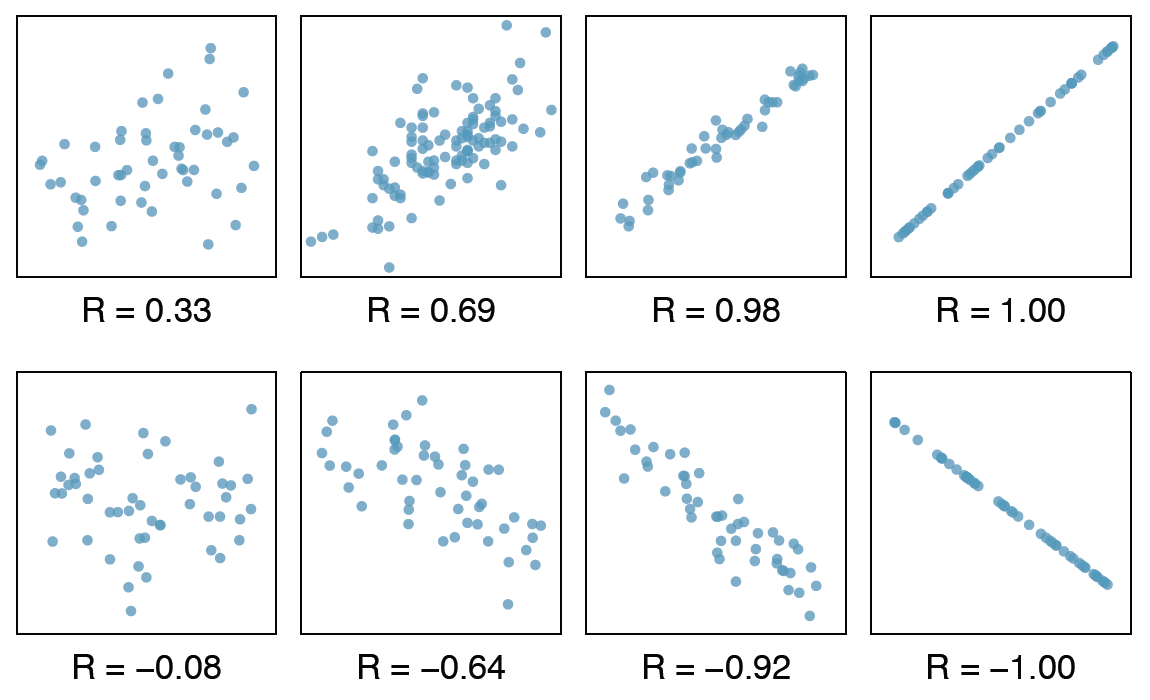
\includegraphics[width=0.7\textwidth]{figure/correlation.png}
\end{center}

\end{frame}
%-------------------------------------------------------------------------------




%-------------------------------------------------------------------------------
\begin{frame}
\frametitle{Best Fitting Line}
\setkeys{Gin}{width=0.75\textwidth}
What does ``best fitting line'' mean?
\begin{center}
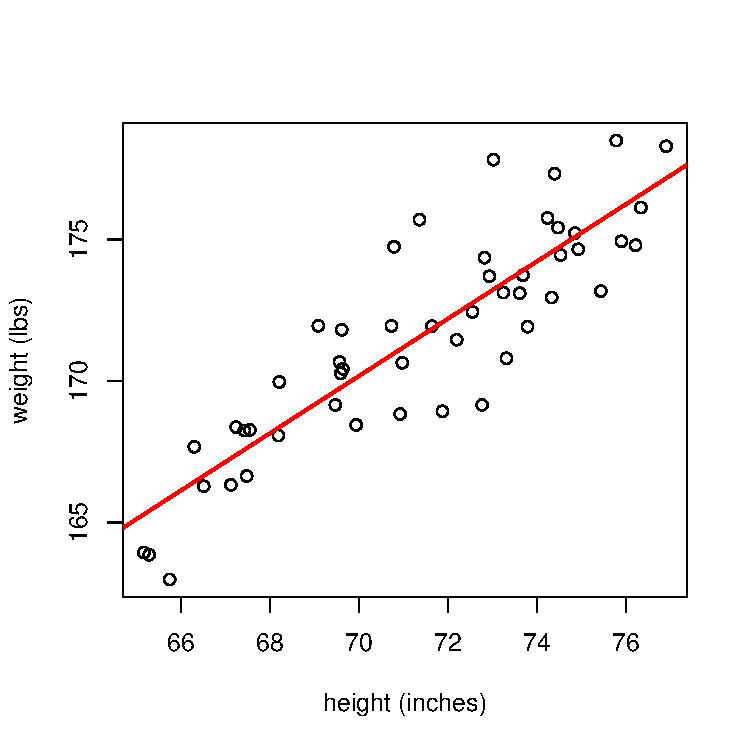
\includegraphics{figure/lec24-003}
\end{center}
\end{frame}
%-------------------------------------------------------------------------------
\begin{frame}
\frametitle{Best Fitting Line}
\setkeys{Gin}{width=0.75\textwidth}
Consider ANY point $x_i$ for $i=1,\ldots,50$ (in blue). 
\begin{center}
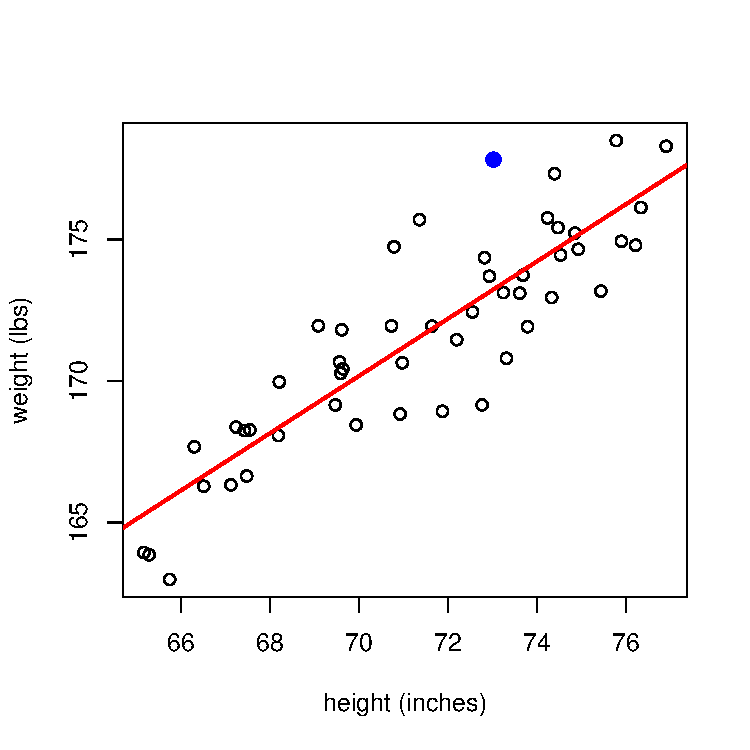
\includegraphics{figure/lec24-004}
\end{center}
\end{frame}
%-------------------------------------------------------------------------------
\begin{frame}
\frametitle{Best Fitting Line}
\setkeys{Gin}{width=0.75\textwidth}
Now consider this point's deviation from the \blue{regression line}
\begin{center}
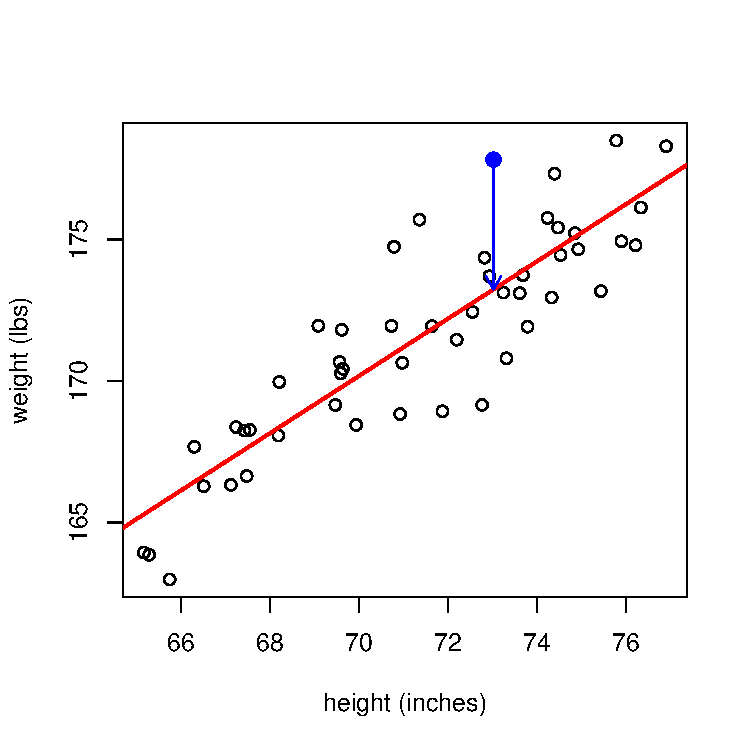
\includegraphics{figure/lec24-005}
\end{center}
\end{frame}
%-------------------------------------------------------------------------------
\begin{frame}
\frametitle{Best Fitting Line}
\setkeys{Gin}{width=0.75\textwidth}
Do this for another point $x_i$\ldots
\begin{center}
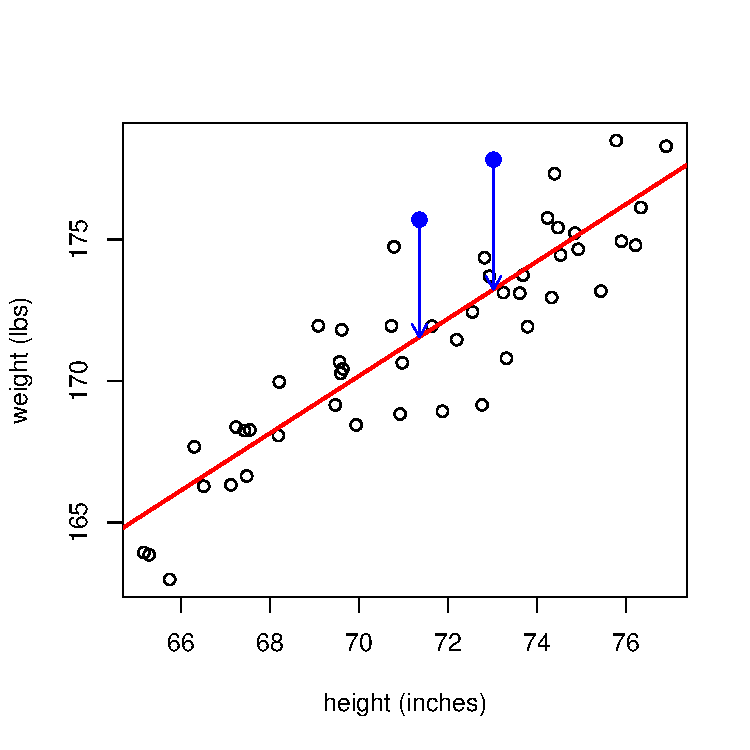
\includegraphics{figure/lec24-006}
\end{center}
\end{frame}
%-------------------------------------------------------------------------------
\begin{frame}
\frametitle{Best Fitting Line}
\setkeys{Gin}{width=0.75\textwidth}
Do this for another point $x_i$\ldots
\begin{center}
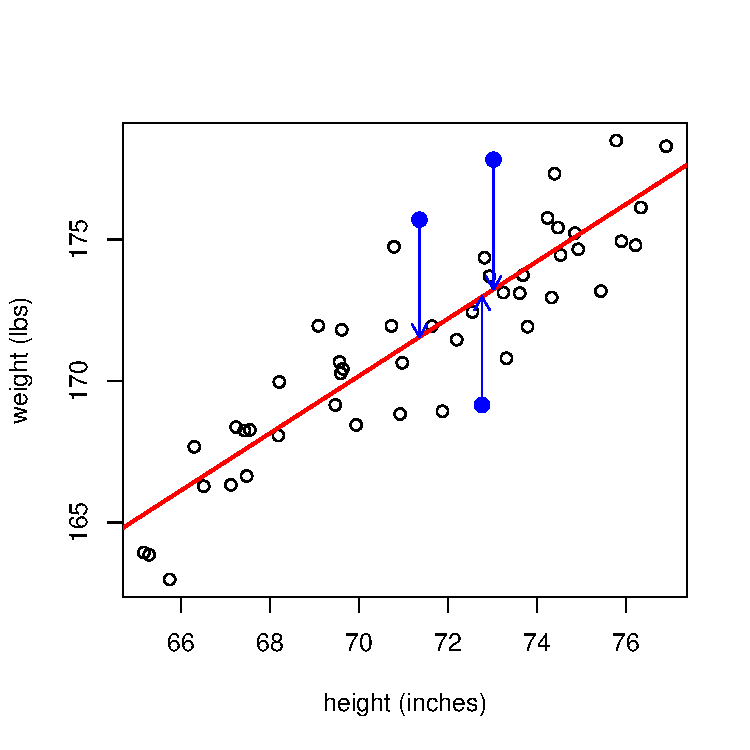
\includegraphics{figure/lec24-007}
\end{center}
\end{frame}
%-------------------------------------------------------------------------------
\begin{frame}
\frametitle{Best Fitting Line}
\setkeys{Gin}{width=0.75\textwidth}
The regression line minimizes the sum of the \blue{squared} arrow lengths.  
\begin{center}
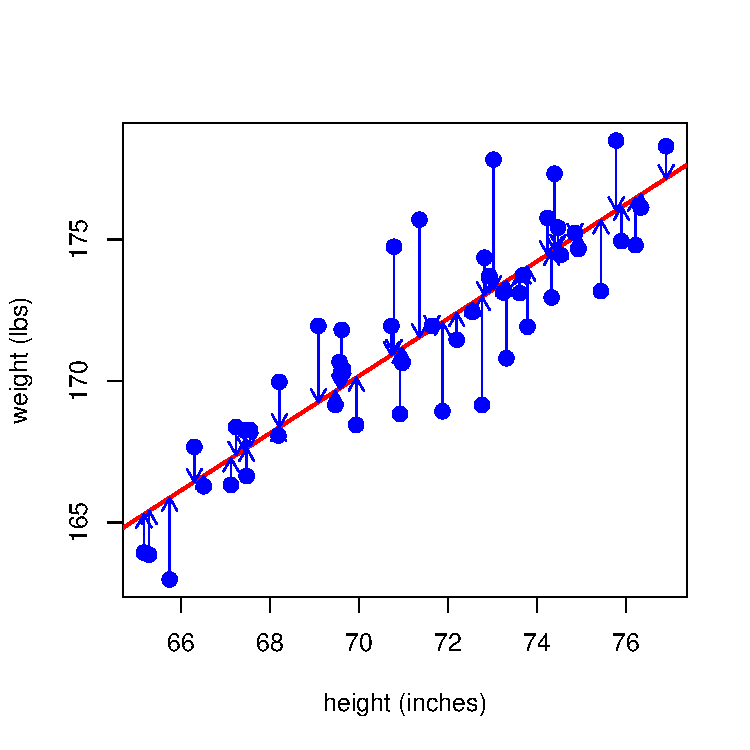
\includegraphics{figure/lec24-008}
\end{center}
\end{frame}
%-------------------------------------------------------------------------------


%------------------------------------------------------------------------------
\begin{frame}[fragile]
\frametitle{Least Squares}
%
% Comment this
%
i.e. the regression line minimizes:
\[
e_1^2 + e_2^2 + \ldots + e_n^2
\]
This is called \blue{minimizing the least squares criterion}.


%\pause Why not minimize
%\[
%|e_1| + |e_2| + \ldots + |e_n| \mbox{ ?}
%\]
%It's easier to do calculus on $x^2$ than $|x|$
\end{frame}
%------------------------------------------------------------------------------


%------------------------------------------------------------------------------
\begin{frame}[fragile]
\frametitle{Conditions for Simple Linear Regression}
%
% Comment this

\begin{itemize}
\pause\item \blue{Linearity}: The data should show a linear trend.  
\pause\item \blue{Independence}: The residuals should be independent
\pause\item \blue{Nearly normal residuals}: The residuals $e_i$ must be nearly normal (verify with QQ-plot) with mean 0.  
\pause\item \blue{Constant variability}:  The variability of points around the least squares line remains roughly constant (i.e. for all values of $x$).
\end{itemize}

\end{frame}
%------------------------------------------------------------------------------


%------------------------------------------------------------------------------
\begin{frame}[fragile]
\frametitle{Behavior of Residuals:  3 Examples}

Sample data + regression on top, residual plots on bottom.  
\begin{center}
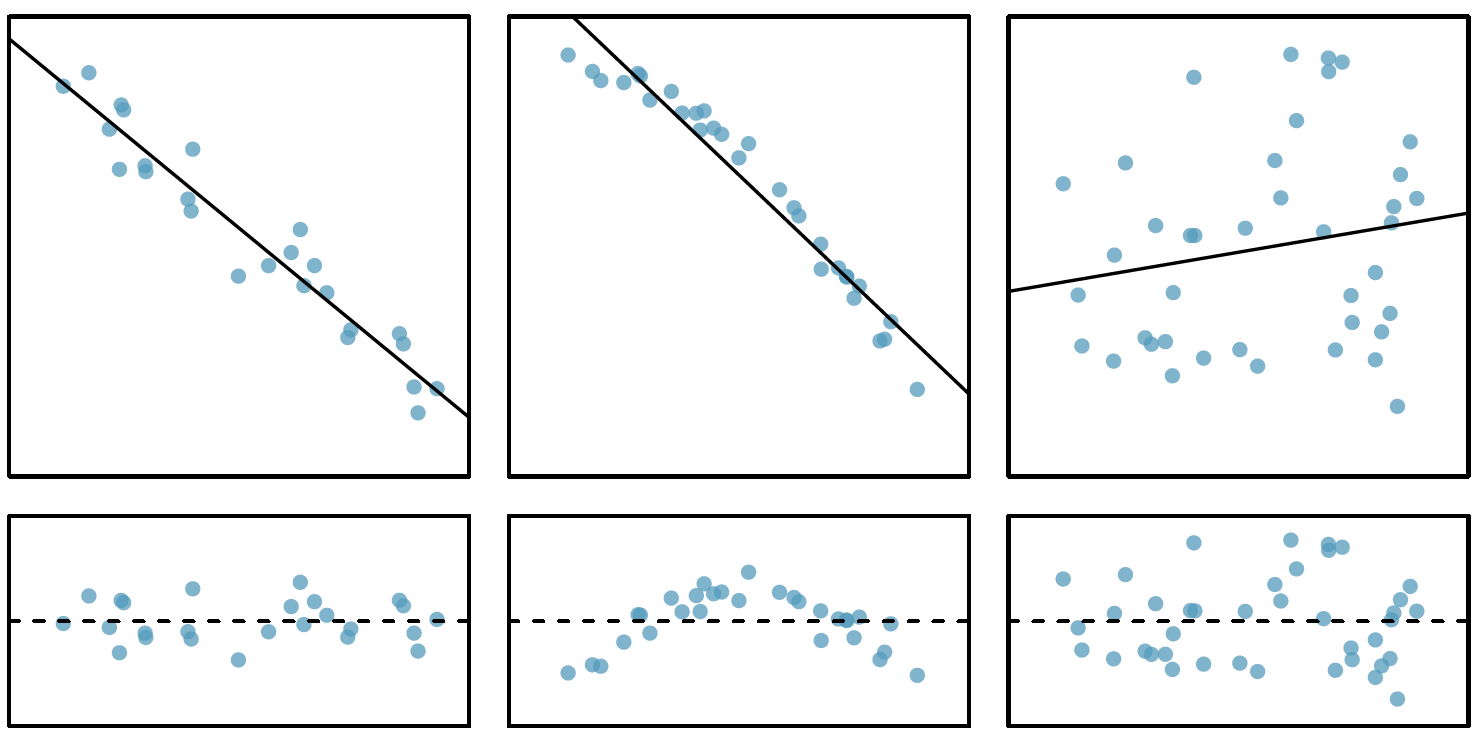
\includegraphics[width=0.8\textwidth]{figure/resid.png}
\end{center}
\begin{itemize}
\pause\item Plots 1 and 3 are roughly linear.
\pause\item Plots 1 and 3 have roughly constant variability, but the 3rd plot has higher variability
\end{itemize}


\end{frame}
%------------------------------------------------------------------------------







%------------------------------------------------------------------------------
\begin{frame}[fragile]
\frametitle{Finding the Least Squares Line}
%
% Comment this
%
To find the least squares line we need to find the point estimates:
\begin{itemize}
\item The point estimate $b_1$ of the slope $\beta_1$ is
\[
b_1 = \frac{s_y}{s_x}R
\]
%where $R$ is the correlation coefficient and $s_y, s_x$ are the sample standard deviations.
\pause\item The regression line \blue{always} goes through $(\xbar, \ybar)$.  We use this fact to find the point estimate of $b_0$ of the intercept $\beta_0$.
\end{itemize}
 
\end{frame}
%------------------------------------------------------------------------------


%------------------------------------------------------------------------------
\begin{frame}[fragile]
\frametitle{Finding the Point Estimate of the Intercept $b_0$}
%
% Comment this
%
Given the slope and a point on the line $(x_0, y_0)$, the equation for the line can be written as 
\begin{eqnarray*}
\mbox{slope} &=& \frac{\mbox{rise}}{\mbox{run}} = \frac{y-y_0}{x-x_0}\\
y-y_0 &=& \mbox{slope} \times (x-x_0)
\end{eqnarray*}

\pause So
\begin{eqnarray*}
&& y - \ybar = b_1(x - \xbar)\\
\mbox{so} && y = \left(\ybar - b_1\xbar\right) + b_1 x\\
\mbox{so} && b_0 = \ybar - b_1\xbar\\
\end{eqnarray*}

\end{frame}
%------------------------------------------------------------------------------


%------------------------------------------------------------------------------
\begin{frame}[fragile]
\frametitle{Measuring the Strength of a Fit}
If $R=-1$ or $R=1$ we have a perfect linear fit between $x$ and $y$, if $R=0$ then there is no fit.
\pause
\vspace{0.5cm}

However $R^2$ is a more commonly used measure of the strength of fit.  For SLR, it is correlation coefficient squared, but not for other kinds of regression.  
\pause

\vspace{0.5cm}
$R^2$ of a linear model describes the \blue{proportion of the total variation in $y$ that is explained by the least squares line}.

\end{frame}
%------------------------------------------------------------------------------


%%------------------------------------------------------------------------------
%\begin{frame}[fragile]
%\frametitle{Height vs Weight Output in R}
%\begin{verbatim}
%lm(formula = height ~ weight)
%
%Residuals:
%    Min      1Q  Median      3Q     Max 
%-3.8231 -1.1495 -0.2926  1.0207  4.5872 
%
%Coefficients:
%            Estimate Std. Error t value Pr(>|t|)    
%(Intercept) 99.39105    5.81100   17.10   <2e-16 ***
%weight       1.01130    0.08131   12.44   <2e-16 ***
%---
%Signif. codes:  0 �***� 0.001 �**� 0.01 �*� 0.05 �.� 0.1 � � 1
%
%Residual standard error: 1.859 on 48 degrees of freedom
%Multiple R-squared:  0.7632,	Adjusted R-squared:  0.7582 
%F-statistic: 154.7 on 1 and 48 DF,  p-value: < 2.2e-16
%\end{verbatim}
%
%\end{frame}
%%------------------------------------------------------------------------------


%------------------------------------------------------------------------------
\begin{frame}[fragile]
\frametitle{Next Time}

\begin{itemize}
\item How to interpret regression line parameter estimates
\item Categorical Variable for $x$:  male vs female, new vs used, etc.
\item Inference for linear regression
\end{itemize}

\end{frame}
%------------------------------------------------------------------------------


%%-------------------------------------------------------------------------------
%\begin{frame}
%\frametitle{Modeling $x$ and $y$ with a Straight Line}
%\blue{The simple linear regression model} assumes that
%\begin{eqnarray*}
%y &=& \underbrace{\beta_0 + \beta_1 x}_{\mbox{non-random}} + \underbrace{\epsilon}_{\mbox{random}}
%\end{eqnarray*}
%\pause This line is called the \blue{true/population regression line} where the 
%$\epsilon$'s are \blue{random deviations} that have normal distribution with $\mu=0$ and standard deviation $\sigma_{\epsilon}$.  \pause i.e. they average out to 0.
%\end{frame}
%%-------------------------------------------------------------------------------


\end{document}










